\documentclass[12pt]{article}
\usepackage{amsmath}
\usepackage{graphicx}
\usepackage{enumerate}
\usepackage{natbib, bbm}
\usepackage{url} % not crucial - just used below for the URL

\usepackage{amsthm}
\usepackage{lipsum}

\usepackage{xparse}
\usepackage{mathtools}
\usepackage[table,dvipsnames]{xcolor}

\usepackage{ifthen}
\usepackage{pstricks}
\usepackage[normalem]{ulem}

\usepackage{booktabs}

\DeclareMathOperator*{\argmin}{arg\,min}
\DeclareMathOperator*{\argmax}{arg\,max}

\newcommand{\kmax}{k_{\text{max}}}
\newcommand{\lambdagrid}{\lambda^{\text{grid}}}

\usepackage{multirow}

\newtheoremstyle{break}
  {\topsep}{\topsep}%
  {\itshape}{}%
  {\bfseries}{}%
  {\newline}{}%
\theoremstyle{break}
\newtheorem{theorem}{Theorem}

\newtheoremstyle{break}
  {\topsep}{\topsep}%
  {\itshape}{}%
  {\bfseries}{}%
  {\newline}{}%
\theoremstyle{break}
\newtheorem{prop}{Proposition}

\newboolean{DEBUG}
\setboolean{DEBUG}{true}
\newrgbcolor{amycolor}{.7 .1 .1}
\ifthenelse {\boolean{DEBUG}}
{\newcommand{\amy}[1]{{\bf \amycolor{[\@Amy: #1]}}}}
{\newcommand{\amy}[1]{}}


\RequirePackage[OT1]{fontenc}
\RequirePackage{amsthm,amsmath, bbm, xspace, graphics, graphicx}
%\RequirePackage{breqn}
%\RequirePackage[colorlinks,citecolor=blue,urlcolor=blue]{hyperref}

\pdfminorversion=4
% NOTE: To produce blinded version, replace "0" with "1" below.
\newcommand{\blind}{1}

% DON'T change margins - should be 1 inch all around.
\addtolength{\oddsidemargin}{-.5in}%
\addtolength{\evensidemargin}{-.5in}%
\addtolength{\textwidth}{1in}%
\addtolength{\textheight}{-.3in}%
\addtolength{\topmargin}{-.8in}%


\begin{document}

%\bibliographystyle{natbib}

\def\spacingset#1{\renewcommand{\baselinestretch}%
{#1}\small\normalsize} \spacingset{1}


%%%%%%%%%%%%%%%%%%%%%%%%%%%%%%%%%%%%%%%%%%%%%%%%%%%%%%%%%%%%%%%%%%%%%%%%%%%%%%


\noindent \textbf{Note from Alex:}\textit{ Included is my data analysis draft, a figure, a table and some blue comments which may or may not be useful in discussion.  I did the table two ways - the same information is contained in both versions (The \texttt{mutlirow} package is needed for the first one.)  As always happy to edit text, figures or tables if that's helpful.}






\section{Data Analysis}
\label{sec:data_analysis}

\subsection{Estimating microbial richness in Lake Champlain}

To illustrate the performance of our methods on ecological data, we estimate strain-level microbial diversity in Lake Champlain, a large eutrophic lake in Canada.  We analyze data from \citet{tromas_2017}, considering samples from the littoral zone in the summer season of the same year as replicates. This gives us 8 replicates from 2009, 6 replicates from 2010 and 6 replicates from 2011.  

The richness estimates from each method are displayed in Figure \ref{fig:data_analysis}.  Method 0 produces the highest estimate for 2009 ($\widehat{C}_{[0]} = 73,404$) and 2010 ($\widehat{C}_{[0]}$ = 47,631) and it was second highest to Method 2 in 2011 ($\widehat{C}_{[2]} = 118,547$).  Method 1 consistently estimated $\widehat{C}$ to be at or near the observed richness, $C_{[1]} = 584$ in 2009,  $572$ in 2010 and $718$ in 2011.  Methods 3 and 4, which both use goodness of fit, were between these two extremes.  These results mirror what we observed in simulations, where Methods 0 and 2 were the highest estimates and Method 1 was the lowest (see Figure \ref{fig:tuning_sim_1}).

These estimates are up to 160 times the observed richness, suggesting that a majority of the species were unobserved in each sample.  The relatively inflated estimates suggest that these data may be poorly fit by the negative binomial model.  \\


\noindent \textcolor{blue}{\textbf{Notes for discussion:}
The reason we model species richness is that the observed richness is an underestimate of the actual richness.  The motivation for penalization is that the unpenalized MLE tends to be much larger than the actual richness.  These results show that only the methods making use of a goodness of fit metric (3 and 4) were consistently between Method 0 and the observed richness in all samples.  We conclude Methods 3 and 4 show the greatest promise on real data containing replicates.}

\textcolor{blue}{
In order to apply our methods to real data, some manual tuning of the optimization search grids ($\lambdagrid$ and the search grid for $C$) was required.} 

\normalsize


\begin{table}[ht]
\caption{Diversity estimates from the Lake Champlain data analysis from 2009 ($r = 8$), 2010 ($r = 6$) and 2011 ($r = 6$) from our proposed methods. 
\label{tab:data_analysis}}
\centering
\begin{tabular}{llcccc}
\toprule
Year & Method & $\widehat{C}$ & $\widetilde{\lambda}$ & $\widehat{\alpha}$ & $\widehat{\delta}$ \\ 
  \midrule
2009 & {[0]} Unpenalized MLE & 73,404 & \textemdash & 0.00088 & 0.00180 \\ 
  \multirow{5}{*} & {[1]} Minimum Variance & 584 & 700 & 0.28863 & 0.00326 \\ 
  \multirow{5}{*} & {[2]} CV Likelihood & 25,930 & 220 & 0.00516 & 0.00142 \\ 
  \multirow{5}{*} & {[3]} Goodness of fit & 20,160 & 550 & 0.00323 & 0.00174 \\ 
  \multirow{5}{*} & {[4]} CV G.O.F. & 39,997 & 100 & 0.00578 & 0.00253 \\ 
  2010 & {[0]} Unpenalized MLE & 47,631 & \textemdash & 0.00185 & 0.00253 \\ 
  \multirow{5}{*} & {[1]} Minimum Variance & 572 & 500 & 0.62668 & 0.00724 \\ 
  \multirow{5}{*} & {[2]} CV Likelihood & 24,799 & 0 & 0.00379 & 0.00270 \\ 
  \multirow{5}{*} & {[3]} Goodness of fit & 13,156 & 220 & 0.00685 & 0.00258 \\ 
  \multirow{5}{*} & {[4]} CV G.O.F. & 47,098 & 0 & 0.00208 & 0.00277 \\ 
  2011 & {[0]} Unpenalized MLE & 57,686 & \textemdash & 0.00161 & 0.00140 \\ 
  \multirow{5}{*} & {[1]} Minimum Variance & 718 & 500 & 0.40112 & 0.00355 \\ 
  \multirow{5}{*} & {[2]} CV Likelihood & 118,547 & 0 & 0.00122 & 0.00193 \\ 
  \multirow{5}{*} & {[3]} Goodness of fit & 40,040 & 230 & 0.00231 & 0.00137 \\ 
  \multirow{5}{*} & {[4]} CV G.O.F. & 36,395 & 5 & 0.00358 & 0.00178 \\ 
   \bottomrule
\end{tabular}
\end{table}

\begin{table}[ht]
\caption{Diversity estimates from the Lake Champlain data analysis from 2009 ($r = 8$), 2010 ($r = 6$) and 2011 ($r = 6$) from our proposed methods. 
\label{tab:data_analysis_compact}}
\centering
\tiny
\begin{tabular}{lllllllllllll}
  \toprule
      & \multicolumn{4}{c}{2009} & \multicolumn{4}{c}{2010} & \multicolumn{4}{c}{2011} \\ \cmidrule(lr){2-5}\cmidrule(lr){6-9}\cmidrule(lr){10-13}
Method & $\widehat{C}$ & $\widetilde{\lambda}$ & $\widehat{\alpha}$ & $\widehat{\delta}$ & $\widehat{C}$ & $\widetilde{\lambda}$ & $\widehat{\alpha}$ & $\widehat{\delta}$ & $\widehat{C}$ & $\widetilde{\lambda}$ & $\widehat{\alpha}$ & $\widehat{\delta}$ \\ 
  \midrule
{[0]} Unpenalized MLE & 73,404 & \textemdash & 0.00088 & 0.00180 & 47,631 & \textemdash & 0.00185 & 0.00253 & 57,686 & \textemdash & 0.00161 & 0.00140 \\ 
  {[1]} Minimum Variance & 584 & 700 & 0.28863 & 0.00326 & 572 & 500 & 0.62668 & 0.00724 & 718 & 500 & 0.40112 & 0.00355 \\ 
  {[2]} CV Likelihood & 25,930 & 220 & 0.00516 & 0.00142 & 24,799 & 0 & 0.00379 & 0.00270 & 118,547 & 0 & 0.00122 & 0.00193 \\ 
  {[3]} Goodness of fit & 20,160 & 550 & 0.00323 & 0.00174 & 13,156 & 220 & 0.00685 & 0.00258 & 40,040 & 230 & 0.00231 & 0.00137 \\ 
  {[4]} CV G.O.F. & 39,997 & 100 & 0.00578 & 0.00253 & 47,098 & 0 & 0.00208 & 0.00277 & 36,395 & 5 & 0.00358 & 0.00178 \\ 
   \bottomrule
\end{tabular}
\end{table}

\begin{figure}[t]
\caption{Estimates of strain-level microbial diversity in Lake Champlain in the summers of 2009 ($r = 8$), 2010 ($r = 6$) and 2011 ($r = 6$) based on our proposed methods.
%$\widehat{C}_{[\text{method}]}$ is the $C$ estimate obtained using the methods defined in Section \ref{sec:tuning_proposals}, shown for each sample.  The number of replicates in each sample is given by $r$.
%
% A visual display of the results from Table \ref{tab:data_analysis}, $\widehat{C}$ estimates from each method.
\label{fig:data_analysis}}
\centering\makebox[\textwidth]{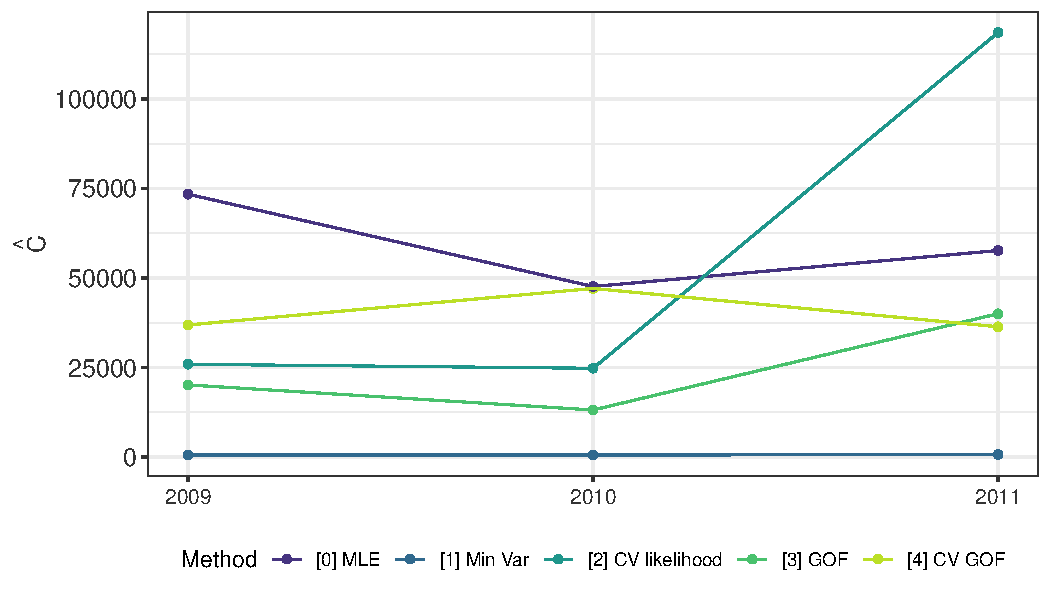
\includegraphics[width=\textwidth]{./images/data_analysis_expanded.pdf}}
\end{figure}


%\bibliographystyle{biorefs}
%\bibliography{refs,amys-papers-library}


\end{document}
